\chapter{Ejemplo \emph{Euler-Lagrange} Rotación 2D}

	
\begin{tikzpicture}
	\fill [left color=red!50, right color=teal!50] (0,0) rectangle (6.5,.1);
	\fill [left color=teal!50, right color=blue!50] (6.5,0) rectangle (11.5,.1);
	\end{tikzpicture}

\vspace{1cm}
\begin{adjustwidth}{50pt}{50pt}
\begin{ejemplo}
Veremos la forma que adopta el lagrangiano para un sistema de partículas en el que no actúan fuerzas externa y que giran entorno al CM (aparece la energía cinética de traslación del CM y la de rotación en torno al CM).
\end{ejemplo}
\end{adjustwidth}

%\vspace{0.5cm}


\section{Ejemplo \emph{Euler-Lagrange} Rotación 2D}
\label{T5ELroracion}

%\vspace{5mm}

\begin{example}

\begin{multicols}{2}
Dos masas $M$ y $m$unidas por una barra rígida de masa despreciable (ligadura).

\vspace{2mm} No hay rozamiento y sobre las masas no actúa ninguna fuerza externa.
	\begin{figure}[H]
		\centering
		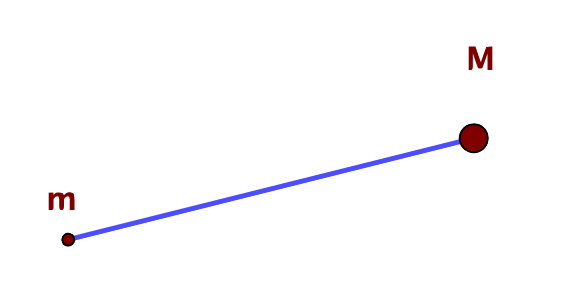
\includegraphics[width=.4\textwidth]{imagenes/img05-01.png}
	\end{figure}
\end{multicols}	
\end{example}

\vspace{3mm}
\ul{Inciso-1} $\quad$ \rule{150pt}{0.1pt} $\quad$ \textbf{Centro de masas.}

Consideremos des masas, $M$ y $m$, sobre una superficie horizontal sin fricción sobre las que no actúa ninguna fuerza neta.
\begin{multicols}{2}
	
	\begin{figure}[H]
		\centering
		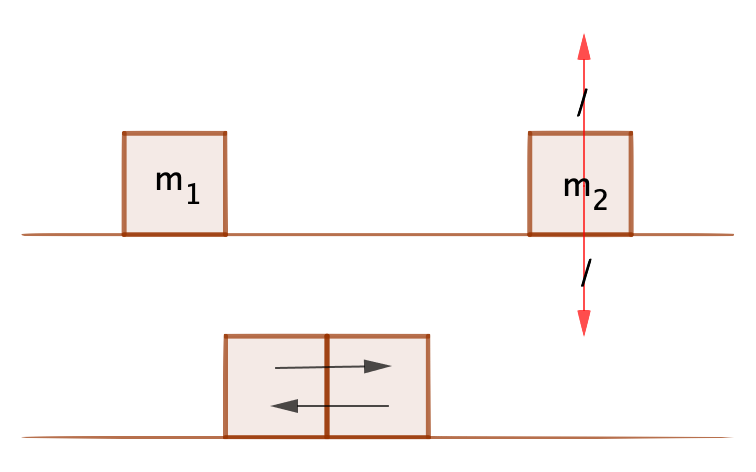
\includegraphics[width=.4\textwidth]{imagenes/img05-02.png}
	\end{figure}
	
	Durante el choque, cada cuerpo nota la fuerza que el orro ejerce sobre él y responde (3a de Newton) con una fuerza igual pero de sentido contrario.
	
$ \overrightarrow F_1=-\overrightarrow F_2 \qquad \ m_1\overrightarrow a_1=-m_2 \overrightarrow a_2	$
\end{multicols}

Integrando: $\ \displaystyle \int m_1 \vec a_1 	\dd t=-\int m_2 \vec a_2 \dd t \ \to \ m_1\vec v_1=-m_2\vec v_2+\overrightarrow A \textcolor{gris}{(\overrightarrow {cte})}$

Volviendo a integrar: $\ \displaystyle \int m_1\vec v_1 \dd t= - \int m_2\vec v_2 \dd t+ \int \overrightarrow A \dd t \ \to \ 
m\vec r_1 = -m_2\vec r_2 +\overrightarrow A t + \overrightarrow B$

Despejando, $\ m\vec r_1 + m_2\vec r_2 = \overrightarrow A t + \overrightarrow B \ \leadsto \ $ dimensiones de [M $\cdot$ L]

Dividiendo por la suma de masas: 
 $\ \dfrac{ m\vec r_1 + m_2\vec r_2}{m_1+m_2} = 
 \dfrac{ \overrightarrow A t + \overrightarrow B} {m_1+m_2} \ \leadsto \ $ dimensiones de [L]
 
 Llamamos $ \ \boldsymbol{ \overrightarrow R(t) \ = \ \dfrac{ m\vec r_1 + m_2\vec r_2}{m_1+m_2} } \quad = \dfrac{\overrightarrow B}{m_1+m_2} + \dfrac{\overrightarrow A}{m_1+m_2} t $
 
 Para $t=0 \ \to \ \overrightarrow R(0)=\dfrac{\overrightarrow B}{m_1+m_2} \ \to \overrightarrow R(t)=\overrightarrow R (0) + \dfrac{\overrightarrow A}{m_1+m_2} \ t \ \leadsto \ $ dimensiones [L], por lo que  $\dfrac{\overrightarrow A}{m_1+m_2} \ \leadsto \ $ dimensiones [LT$^{-1}$], con lo que llamamos $\ \overrightarrow V = \dfrac{\overrightarrow A}{m_1+m_2} $
 
 Finalmente: 
 
 \begin{equation}
 \overrightarrow R(t) \ = \ \overrightarrow R(0) \ + \ \overrightarrow V \ t	
 \end{equation}
 
 Dos masas sobre las que no actúa ninguna fuerza externa, solo actúan fuerzas internas (como en el momento del choque) aparece un vector $\overrightarrow R$ que viaja con MRU \textcolor{gris}{(movimiento rectilíneo y uniforme)}. $\overrightarrow R$ es la \textbf{posición del \emph{centro de masas}} y $\overrightarrow V$ es la \textbf{velocidad del \emph{centro de masas}}: $\ \overrightarrow R=\overrightarrow R_{CM};\ \ \overrightarrow V=\overrightarrow V_{CM}$
 
 Por ello, $\ \boldsymbol{ \overrightarrow V= }\displaystyle \dv{t} \overrightarrow R = \boldsymbol{ \dfrac{m_1\vec v_1 + m_2 \vec v_2}{m_1+m_2} }$
 
 Todo esto es generalizable al caso de N partículas:
 
 \begin{equation}
 \boldsymbol{
 \overrightarrow R \ =  \  \dfrac{ \displaystyle \sum_{i=1}^N m_i \ \vec r_i	}{ \displaystyle \sum_{i=1}^N m_i} \, ; \qquad  \qquad
  \overrightarrow V \ =  \  \dfrac{ \displaystyle \sum_{i=1}^N m_i \ \vec v_i	}{\displaystyle \sum_{i=1}^N m_i}
  }
 \end{equation}

\begin{flushright} \rule{300pt}{0.1pt}	\end{flushright}



	\begin{figure}[H]
	\centering
	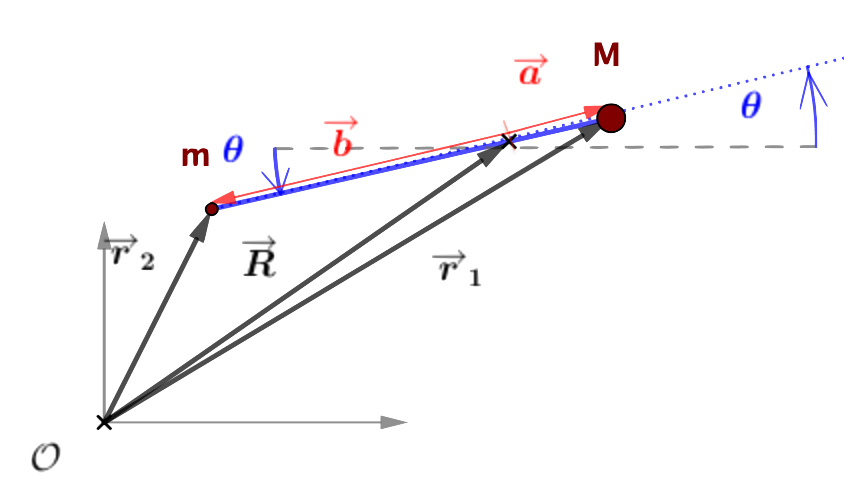
\includegraphics[width=.6\textwidth]{imagenes/img05-03.png}
	\end{figure}
	


Vamos a por el lagrangiano, en nuestro caso, $ \ L=T-\cancel{V}=T =T_1+T_2\, , \ $  \textcolor{gris}{($\  \nexists  \overrightarrow F^{ext}$ )}

$\begin{cases}
\ \vec r_1 = \overrightarrow R + \vec a  \to \vec v_1= \overrightarrow V + \dot{\vec a}
\\ \ \vec r_2=\overrightarrow R + \vec b	 \to \vec v_2=\overrightarrow V + \dot{\vec b}
\end{cases}  $

$\begin{cases} 
\ \vec a=a(\cos \theta, \sin \theta) \quad \ \ \to \ \dot{\vec a}=a\dot \theta (-\sin \theta,\cos \theta ) \ \to \ |\vec a|^2=a^2 \dot \theta^2 \\
\ \vec b=b(-\cos \theta, -\sin \theta)  \to \ \dot{\vec b}=b\dot \theta (sin \theta,-\cos \theta ) \ \, \to \ |\vec b|^2=b^2 \dot \theta^2 
\end{cases}$ \begin{footnotesize} $\ \  \textcolor{gris}{(\sin^2 \theta + …\cos^2 \theta=1)}$ \end{footnotesize}

$\begin{cases}
\ v_1^2=V^2+|\vec a|^2+2\vec v \cdot \dot{\vec a} \\	
\ v_2^2=V^2+|\vec b|^2+2\vec v \cdot \dot{\vec b}
\end{cases} \quad \to \qquad T=\dfrac M 2 \ v_1^2 + \dfrac m 2 \ v_2^2$ 

$T=\dfrac 1 2 {(M+m)} V^2 + \dfrac M 2 |\dot{\vec a}|^2 + \dfrac m 2 |\dot{ \vec b}|^2 + M \overrightarrow V \cdot \dot{\vec a}+ m \overrightarrow V \cdot \dot{\vec b} $

$T=\dfrac 1 2 {(M+m)} V^2 + \dfrac M 2 |\dot{\vec a}|^2 + \dfrac m 2 |\dot {\vec b}|^2 +\overrightarrow V \cdot (M\dot{\vec a} + m\dot{\vec b})$

$T=\dfrac 1 2 {(M+m)} V^2 + \dfrac M 2 |\dot{\vec a}|^2 + \dfrac m 2 |\dot {\vec b}|^2 +
\overrightarrow V \cdot \cancelto{0}{ \displaystyle \dv{t} (M \vec a + m \vec b)}$

\vspace{7mm} 
\ul{Inciso-2} $\quad$ \rule{150pt}{0.1pt} $\quad$ 

$V \cdot  \displaystyle \dv{t} (M \vec a + m \vec b) = 
V \cdot  \displaystyle \dv{t} [M (\vec r_1-\overrightarrow R) + m (\vec r_2-\overrightarrow R)]=
V \cdot  \displaystyle \dv{t} [M\vec r_1+m\vec r_2 - (M+m) \overrightarrow R ]=
V \cdot  \displaystyle \dv{t} [M\vec r_1+m\vec r_2 - \cancel{(M+m)} \dfrac{M\vec r_1 + m \vec r_2}{ \cancel{M+m}}]=
V \cdot \displaystyle \dv{t} \ 0 =0$

\begin{flushright} \rule{300pt}{0.1pt}	\end{flushright}

\vspace{5mm}

Luego, $ \ T=\dfrac 1 2 {(M+m)} V^2 + \dfrac M 2 |\dot{\vec a}|^2 + \dfrac m 2 |\dot {\vec b}|^2$

Sustituyendo los valores obtenidos para $|\dot{\vec a}|^2 \text{ y } |\dot{\vec b}|^2 $,

$L=T=\dfrac 1 2 {(M+m)} V^2 + \left[ \dfrac M 2 a^2 + \dfrac m 2 b^2 \right] \ \dot \theta^2 =
\dfrac 1 2 {(M+m)} V^2 + \dfrac 1 2 \left[  M  a^2 +  m  b^2 \right] \ \dot \theta^2$

\begin{equation}
\subrayado{ \boxed{ \ \boldsymbol{
 L \ = \ \dfrac 1 2 \ {(M+m)} \ V^2 \ + \ \dfrac 12 \ I_{CM} \ \omega^2
  } \  } }
 \end{equation}
 
 donde $\ I_{CM}\ $ es el \emph{momento de inercia} respecto el centro de masas.

\vspace{5mm}	
\ul{Inciso-3} $\quad$ \rule{150pt}{0.1pt} $\quad$ \textbf{Momento de inercia}

\begin{multicols}{2}
En MCU \begin{footnotesize}  (movimiento circular uniforme) \end{footnotesize}

$\overrightarrow L=\vec r \times \vec p = \vec r \times m \vec v$

$|\overrightarrow L |=rmv \sin \dfrac \pi 2 =m\ r \ v$

$v=\omega r \to L=mr\omega r=(mr^2)\  \omega$
\begin{figure}[H]
	\centering
	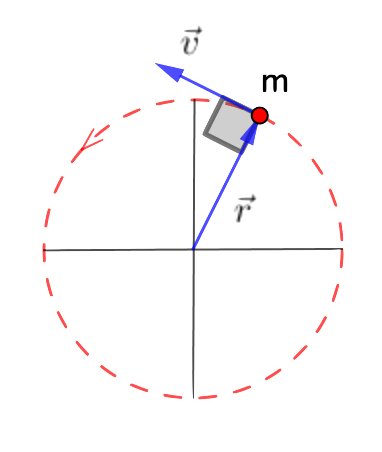
\includegraphics[width=.25\textwidth]{imagenes/img05-06.png}
	\end{figure}	
\end{multicols}

El factor $mr^2\ $ depende de la geometría del sistema y se llama \textbf{\emph{Momento de Inercia}}

	

\vspace{5mm}
Para N partículas ligadas girando en torno al CM con la misma $\omega$,

$$\boldsymbol{}I\ = \ \dfrac{\displaystyle \sum_{i=1}^N m_i \ r_i^2}{\displaystyle \sum_{i=1}^N m_i}\, ; \qquad L \ = \ I \ \omega$$
\begin{flushright} \rule{300pt}{0.1pt}	\end{flushright}

\vspace{5mm}

\begin{myalertblock}{Lagrangiano con rotación}
\begin{large}
\begin{equation}
\label{T5Lconrotacion}
\boldsymbol{
L \ = \ \dfrac{M_{TOTAL}}{2}\ \ V_{CM}^2 \ + \ \dfrac 1 2 \ I_{CM}\  \ \dot \theta^2
} 
\end{equation}	
\end{large}
\end{myalertblock}

Forma que adopta el lagrangiano para un sistema de partículas en el que no actúan fuerzas externa y que giran entorno al CM (aparece la energía cinética de traslación del CM y la de rotación en torno al CM).

	

	
	
	
	
	







